\documentclass{article}

\usepackage{graphicx}
\usepackage{subcaption}
\usepackage[portrait]{geometry}
\geometry{total={8.5in,11in},left=0.25in, top=0.25in, right=0.25in}

\begin{document}

\begin{figure}[h!]
\centering
\begin{subfigure}[b]{0.35\linewidth}
  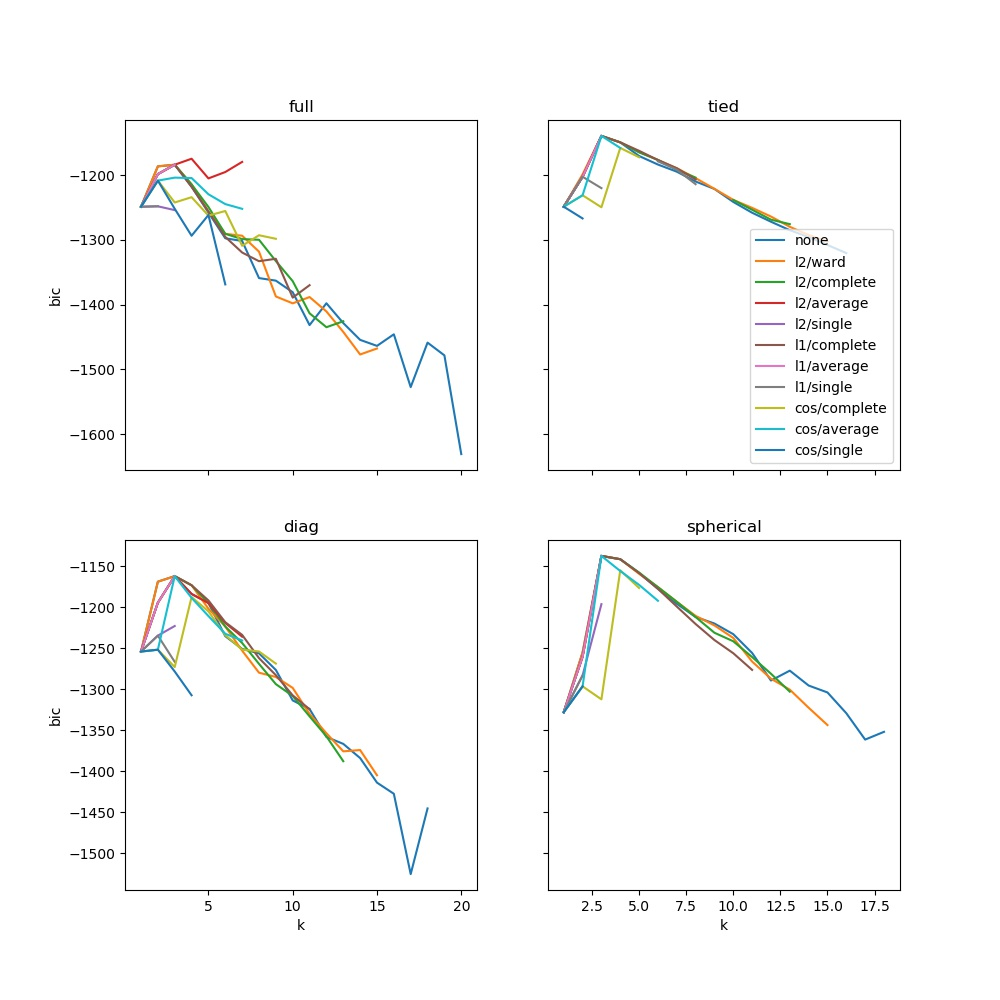
\includegraphics[width=\linewidth]{lowd_python_bicplot.jpg}
\caption{}
\end{subfigure}
\begin{subfigure}[b]{0.35\linewidth}
  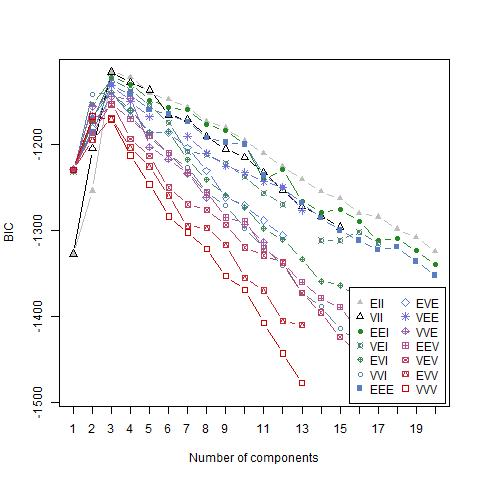
\includegraphics[width=\linewidth]{lowd_r_bicplot.jpg}
\caption{}
\end{subfigure} 
\begin{subfigure}[b]{0.35\linewidth}
  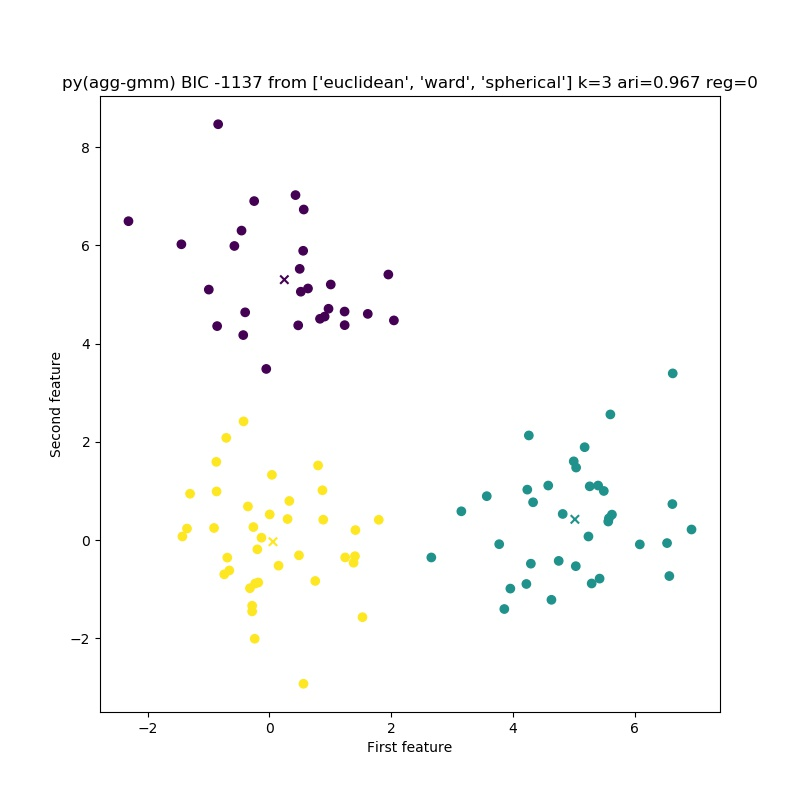
\includegraphics[width=\linewidth]{lowd_python_bestbic.jpg}
\caption{}
\end{subfigure}
\begin{subfigure}[b]{0.35\linewidth}
  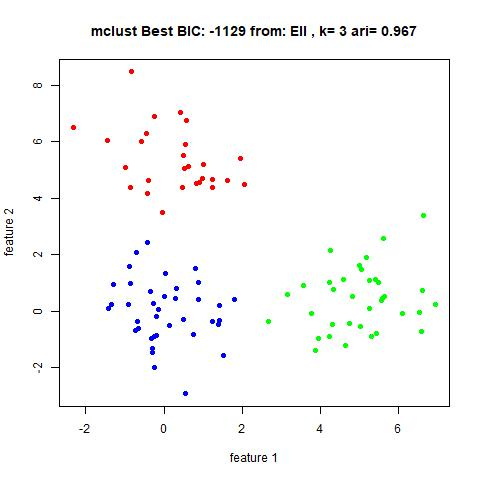
\includegraphics[width=\linewidth]{lowd_r_bestbic.jpg}
\caption{}
\end{subfigure} 

\caption{Results on a simple mixture of 3 Gaussians in 3d. The mixtures have identity covariance and have means at [0,0...],[5,0...],[0,5...]. a) pyclust bicplot b) mclust bicplot c) pyclust clustering with best BIC d) mclust clustering with best BIC}
\end{figure}



\begin{figure}[h!]
\centering
\begin{subfigure}[b]{0.35\linewidth}
  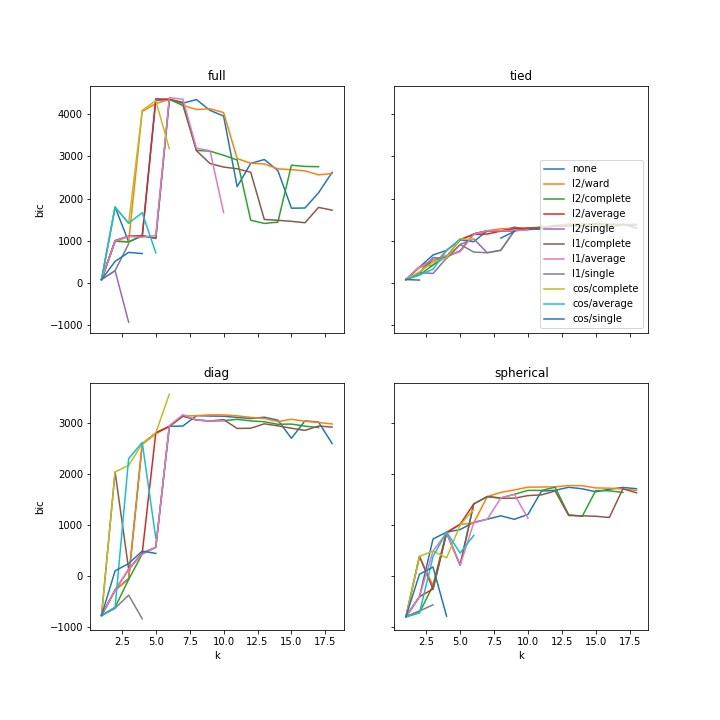
\includegraphics[width=\linewidth]{drosophila_python_bicplot.jpg}
\caption{}
\end{subfigure}
\begin{subfigure}[b]{0.35\linewidth}
  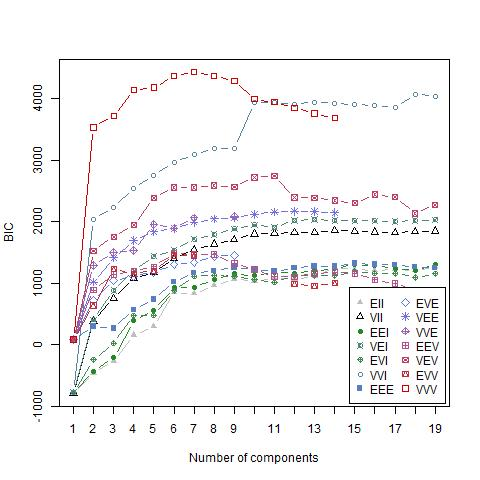
\includegraphics[width=\linewidth]{drosophila_r_bicplot.jpg}
\caption{}
\end{subfigure} 
\begin{subfigure}[b]{0.35\linewidth}
  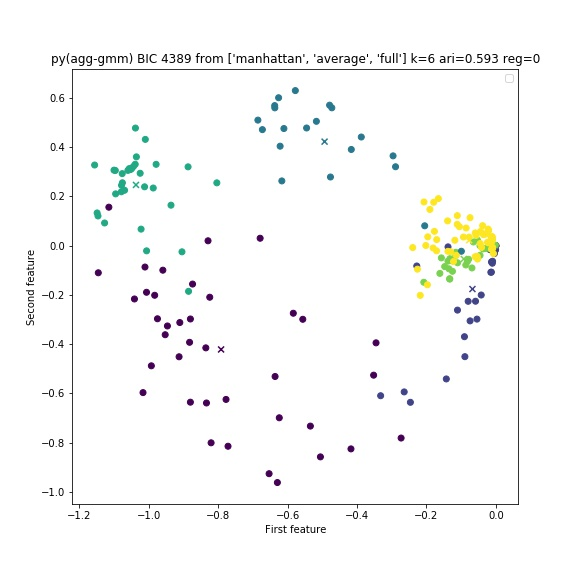
\includegraphics[width=\linewidth]{drosophila_python_bestbic.jpg}
\caption{}
\end{subfigure}
\begin{subfigure}[b]{0.35\linewidth}
  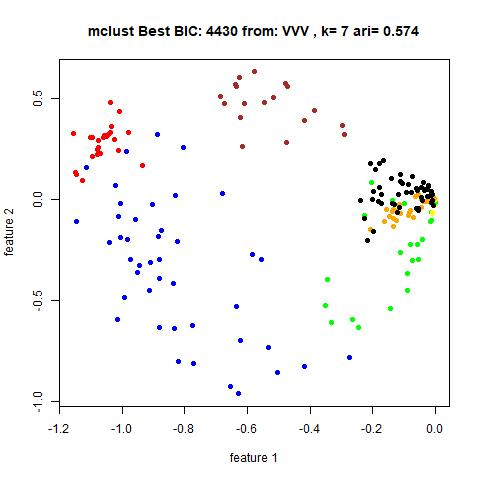
\includegraphics[width=\linewidth]{drosophila_r_bestbic.jpg}
\caption{}
\end{subfigure} 

\caption{Results on embedded Drosophila data}
\end{figure}

\begin{figure}[h!]
\centering
\begin{subfigure}[b]{0.35\linewidth}
  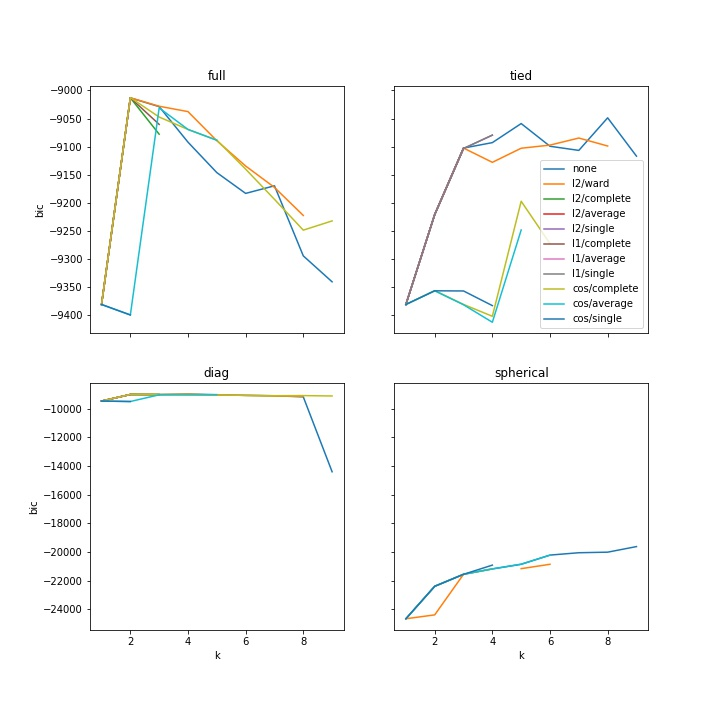
\includegraphics[width=\linewidth]{bc_python_bicplot.jpg}
\caption{}
\end{subfigure}
\begin{subfigure}[b]{0.35\linewidth}
  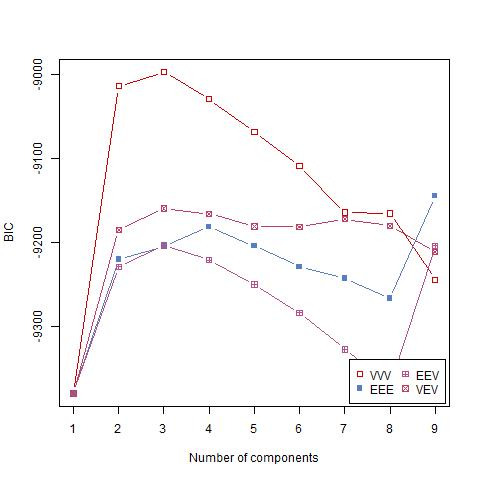
\includegraphics[width=\linewidth]{bc_r_bicplot.jpg}
\caption{}
\end{subfigure} 
\begin{subfigure}[b]{0.35\linewidth}
  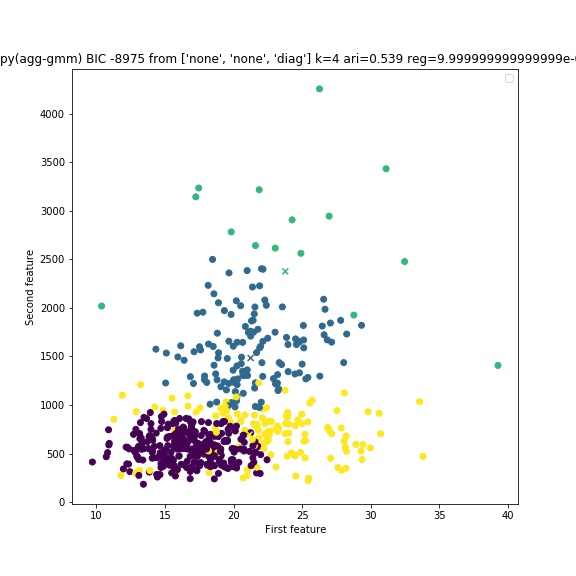
\includegraphics[width=\linewidth]{bc_python_bestbic.jpg}
\caption{}
\end{subfigure}
\begin{subfigure}[b]{0.35\linewidth}
  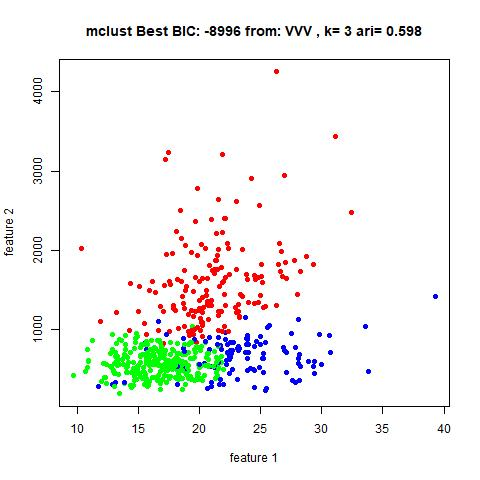
\includegraphics[width=\linewidth]{bc_r_bestbic.jpg}
\caption{}
\end{subfigure} 

\caption{Results on embedded Wisconsin Breast Cancer data}
\end{figure}


\end{document}